\documentclass[11pt]{article}

% Mandatory Packages
\usepackage{amsmath}
\usepackage{amssymb}
\usepackage{amsthm}
\usepackage{geometry}
\usepackage{tikz}
\usetikzlibrary{arrows.meta, positioning, shapes}
\usepackage{mathrsfs}
\usepackage{mathtools}

% Formatting
\geometry{letterpaper, margin=1in}
\setlength{\parindent}{0pt}
\setlength{\parskip}{0.5em}

% Theorem Environments
\newtheorem{theorem}{Theorem}[section]
\newtheorem{lemma}[theorem]{Lemma}
\newtheorem{definition}[theorem]{Definition}
\newtheorem{corollary}[theorem]{Corollary}
\newtheorem{problem}{Problem}
\newtheorem{flawprob}{Diagnostic Problem}

% Title block
\title{\textbf{Homework 4: Proofs Involving Congruence of Integers}}
\author{Tashfeen Omran}
\date{September 2026}

\begin{document}

\maketitle
\tableofcontents
\newpage

% ==========================================
% PART 1: Comprehensive Introduction
% ==========================================
\section{Part 1: Comprehensive Introduction, Context, and Prerequisites}

\subsection{Core Concepts \& Axioms}
In abstract mathematics, the notion of equivalence is fundamental to classifying objects with shared structures. Congruence of integers provides a formal framework for understanding divisibility by establishing an equivalence relation on the set of integers, $\mathbb{Z}$. 

\begin{definition}[Congruence Modulo $n$]
For integers $a$, $b$, and $n \ge 2$, we say that $a$ is congruent to $b$ modulo $n$, denoted as $a \equiv b \pmod n$, if $n$ divides the difference $(a - b)$. 
Formally:
\[ a \equiv b \pmod n \iff n \mid (a - b) \iff \exists k \in \mathbb{Z} : a - b = nk \]
\end{definition}

This definition explicitly bridges divisibility with algebraic manipulation. When two numbers are congruent modulo $n$, they share the same remainder upon division by $n$ (via the Division Algorithm). This effectively partitions $\mathbb{Z}$ into $n$ distinct, mutually exclusive subsets known as \textit{residue classes} or \textit{equivalence classes}, forming the quotient set $\mathbb{Z} / n\mathbb{Z}$.

\subsection{Intuition and Set-Theoretic/Logical Foundations}
Intuitively, modular arithmetic operates like a clock. On a standard 12-hour clock, 13:00 is mathematically treated as 1:00 because $13 \equiv 1 \pmod{12}$. In set-theoretic terms, a congruence relation modulo $n$ is an \textit{equivalence relation} because it satisfies three axioms:
1. \textbf{Reflexivity}: $a \equiv a \pmod n$ (since $n \mid 0$).
2. \textbf{Symmetry}: If $a \equiv b \pmod n$, then $b \equiv a \pmod n$.
3. \textbf{Transitivity}: If $a \equiv b \pmod n$ and $b \equiv c \pmod n$, then $a \equiv c \pmod n$.

This equivalence relation maps the infinite space of $\mathbb{Z}$ into a finite probability space or state space when used in finite-state machines, generating an algebraic structure called a \textit{ring} over the set $\mathbb{Z}_n = \{[0], [1], \dots, [n-1]\}$.

\subsection{Historical Context and Motivation}
The rigorous formalization of modular arithmetic was introduced by the legendary mathematician Carl Friedrich Gauss in his monumental 1801 treatise, \textit{Disquisitiones Arithmeticae}. Before Gauss, mathematicians like Fermat and Euler studied properties of divisibility ad-hoc. Gauss unified these properties under the notation ``$\equiv$'', intentionally mirroring the ``$=$'' sign to signify that congruence behaves algebraically just like equality, resolving structural ambiguities in number theory and paving the way for modern abstract algebra.

\subsection{Key Theorems, Lemmas, and Formulas}
The following theorems form the bedrock of manipulations over $\mathbb{Z} / n\mathbb{Z}$:

\begin{theorem}[Algebraic Properties of Congruence]
Let $a, b, c, d, n \in \mathbb{Z}$ with $n \ge 2$. If $a \equiv b \pmod n$ and $c \equiv d \pmod n$, then:
\begin{enumerate}
    \item \textbf{Translation:} $a + c \equiv b + d \pmod n$
    \item \textbf{Scaling:} $ac \equiv bd \pmod n$
    \item \textbf{Scalar Multiplication:} $ka \equiv kb \pmod n$ for any integer $k$.
    \item \textbf{Exponentiation:} $a^m \equiv b^m \pmod n$ for any positive integer $m$.
\end{enumerate}
\end{theorem}

\subsection{Prerequisites}
To fully master this section, a student must possess:
\begin{itemize}
    \item \textbf{Set Theory Foundation:} Understanding partitions and equivalence classes.
    \item \textbf{Logic:} Comfort with biconditionals ($P \iff Q$) and proof by cases.
    \item \textbf{Basic Divisibility:} The Division Algorithm ($a = qn + r$ with $0 \le r < n$).
    \item \textbf{Proof Techniques:} Mastery of Direct Proof and algebraic substitution.
\end{itemize}

% ==========================================
% PART 2: Detailed Homework Solutions
% ==========================================
\newpage
\section{Part 2: Detailed Homework Solutions}

As per the directive for maximum learning efficiency, a strategic selection of six distinct problem archetypes from Section 4.2 has been made. This sample guarantees rigorous coverage of every underlying theoretical concept without redundant repetition.

\begin{problem}[4.14 - Transitivity in Exponentiation]
Let $a, b, n \in \mathbb{Z}$, where $n \ge 2$. Prove that if $a \equiv b \pmod n$, then $a^2 \equiv b^2 \pmod n$.
\end{problem}
\begin{proof}
\textbf{Proof Technique: Direct Proof.} \\
Let $a, b, n \in \mathbb{Z}$ with $n \ge 2$. Assume that $a \equiv b \pmod n$. 
By the definition of congruence, this implies that $n \mid (a - b)$. 
Therefore, there exists some integer $k$ such that:
\[ a - b = nk \]
We wish to show that $a^2 \equiv b^2 \pmod n$, which requires proving that $n \mid (a^2 - b^2)$.
Consider the expression $a^2 - b^2$. By the algebraic difference of squares, we have:
\[ a^2 - b^2 = (a - b)(a + b) \]
Substitute $a - b = nk$ into the equation:
\[ a^2 - b^2 = (nk)(a + b) = n(k(a + b)) \]
Since $k, a,$ and $b$ are all integers, their combination under addition and multiplication, $k(a+b)$, is also an integer. Let $m = k(a+b)$, where $m \in \mathbb{Z}$. Then:
\[ a^2 - b^2 = nm \]
By definition of divisibility, this shows that $n \mid (a^2 - b^2)$. Therefore, $a^2 \equiv b^2 \pmod n$.
\end{proof}

\begin{problem}[4.15 - Chain Transitivity]
Let $a, b, c, n \in \mathbb{Z}$, where $n \ge 2$. Prove that if $a \equiv b \pmod n$ and $b \equiv c \pmod n$, then $a \equiv c \pmod n$.
\end{problem}
\begin{proof}
\textbf{Proof Technique: Direct Proof.} \\
Assume $a, b, c, n \in \mathbb{Z}$ with $n \ge 2$, such that $a \equiv b \pmod n$ and $b \equiv c \pmod n$. 
By definition, there exist integers $x$ and $y$ such that:
\begin{align}
    a - b &= nx \label{eq1} \\
    b - c &= ny \label{eq2}
\end{align}
We seek to demonstrate that $a \equiv c \pmod n$, meaning $a - c$ is a multiple of $n$.
By adding equation (\ref{eq1}) and equation (\ref{eq2}), we obtain:
\[ (a - b) + (b - c) = nx + ny \]
Simplifying the left-hand side yields:
\[ a - c = n(x + y) \]
Since $x$ and $y$ are integers, their sum $(x + y)$ is an integer. Thus, $n \mid (a - c)$, which means $a \equiv c \pmod n$.
\end{proof}

\begin{problem}[4.16 - Biconditional Congruence / Diophantine Equivalence]
Let $a, b \in \mathbb{Z}$. Prove that $a^2 + 2b^2 \equiv 0 \pmod 3$ if and only if either $a$ and $b$ are both congruent to $0 \pmod 3$ or neither is congruent to $0 \pmod 3$.
\end{problem}
\begin{proof}
\textbf{Proof Technique: Exhaustive Proof by Cases (for both directions).} \\
Let $P$ be the proposition ``$a^2 + 2b^2 \equiv 0 \pmod 3$''. Let $Q$ be the proposition ``$(a \equiv 0 \pmod 3 \land b \equiv 0 \pmod 3) \lor (a \not\equiv 0 \pmod 3 \land b \not\equiv 0 \pmod 3)$''. We must prove $P \iff Q$.

\textit{Preliminary Lemma:} By the Division Algorithm, any integer $x$ modulo 3 falls into exactly one of three cases: $x \equiv 0, 1, \text{ or } 2 \pmod 3$. 
\begin{itemize}
    \item If $x \equiv 0 \pmod 3$, then $x^2 \equiv 0^2 \equiv 0 \pmod 3$.
    \item If $x \equiv 1 \pmod 3$, then $x^2 \equiv 1^2 \equiv 1 \pmod 3$.
    \item If $x \equiv 2 \pmod 3$, then $x^2 \equiv 2^2 \equiv 4 \equiv 1 \pmod 3$.
\end{itemize}
Thus, $x^2 \equiv 0 \pmod 3$ if $x \equiv 0 \pmod 3$, and $x^2 \equiv 1 \pmod 3$ if $x \not\equiv 0 \pmod 3$.

\textbf{Part 1: Show $Q \implies P$} \\
Assume $Q$ is true. We have two sub-cases:
\textit{Sub-case 1.1:} $a \equiv 0 \pmod 3$ and $b \equiv 0 \pmod 3$. 
Then $a^2 \equiv 0 \pmod 3$ and $b^2 \equiv 0 \pmod 3$. 
Evaluating the expression: $a^2 + 2b^2 \equiv 0 + 2(0) \equiv 0 \pmod 3$.
\textit{Sub-case 1.2:} $a \not\equiv 0 \pmod 3$ and $b \not\equiv 0 \pmod 3$. 
From our lemma, $a^2 \equiv 1 \pmod 3$ and $b^2 \equiv 1 \pmod 3$.
Evaluating the expression: $a^2 + 2b^2 \equiv 1 + 2(1) \equiv 3 \equiv 0 \pmod 3$.
In both sub-cases, $P$ is true.

\textbf{Part 2: Show $P \implies Q$ (by contrapositive)} \\
We prove $\sim Q \implies \sim P$. The negation $\sim Q$ is: ``Exactly one of $a$ or $b$ is congruent to $0 \pmod 3$.''
\textit{Sub-case 2.1:} $a \equiv 0 \pmod 3$ and $b \not\equiv 0 \pmod 3$. 
Then $a^2 \equiv 0 \pmod 3$ and $b^2 \equiv 1 \pmod 3$.
Evaluating: $a^2 + 2b^2 \equiv 0 + 2(1) \equiv 2 \not\equiv 0 \pmod 3$.
\textit{Sub-case 2.2:} $a \not\equiv 0 \pmod 3$ and $b \equiv 0 \pmod 3$. 
Then $a^2 \equiv 1 \pmod 3$ and $b^2 \equiv 0 \pmod 3$.
Evaluating: $a^2 + 2b^2 \equiv 1 + 2(0) \equiv 1 \not\equiv 0 \pmod 3$.
Since both sub-cases of $\sim Q$ yield $\sim P$, the contrapositive is proven. Thus $P \iff Q$.
\end{proof}

\begin{problem}[4.18 - Modulus Divisibility]
Let $m, n \in \mathbb{N}$ such that $m \mid n$. Prove that if $a$ and $b$ are integers such that $a \equiv b \pmod n$, then $a \equiv b \pmod m$.
\end{problem}
\begin{proof}
\textbf{Proof Technique: Direct Proof.} \\
Assume $m, n \in \mathbb{N}$ and $m \mid n$. By definition, there exists an integer $k_1$ such that:
\[ n = mk_1 \]
Assume further that $a \equiv b \pmod n$. By definition, there exists an integer $k_2$ such that:
\[ a - b = nk_2 \]
Substitute $n = mk_1$ into the expression for $a - b$:
\[ a - b = (mk_1)k_2 = m(k_1 k_2) \]
Since $k_1$ and $k_2$ are integers, their product $k_1 k_2$ is an integer. Let $j = k_1 k_2$, where $j \in \mathbb{Z}$.
\[ a - b = mj \]
This implies $m \mid (a - b)$, which by definition means $a \equiv b \pmod m$.
\end{proof}

\begin{problem}[4.19 - Linear Congruence Combinations]
Let $a, b \in \mathbb{Z}$. Show that if $a \equiv 5 \pmod 6$ and $b \equiv 3 \pmod 4$, then $4a + 6b \equiv 6 \pmod 8$.
\end{problem}
\begin{proof}
\textbf{Proof Technique: Direct Algebraic Manipulation.} \\
Assume $a \equiv 5 \pmod 6$ and $b \equiv 3 \pmod 4$. By definition, there exist integers $x, y$ such that:
\begin{align}
    a - 5 &= 6x \implies a = 6x + 5 \\
    b - 3 &= 4y \implies b = 4y + 3 
\end{align}
We want to evaluate $4a + 6b$ modulo 8. Substitute our expressions for $a$ and $b$ into $4a + 6b$:
\begin{align*}
    4a + 6b &= 4(6x + 5) + 6(4y + 3) \\
            &= 24x + 20 + 24y + 18 \\
            &= 24x + 24y + 38
\end{align*}
To determine the congruence modulo 8, we extract multiples of 8:
\begin{align*}
    24x + 24y + 38 &= 8(3x) + 8(3y) + 32 + 6 \\
                   &= 8(3x + 3y + 4) + 6
\end{align*}
Since $x$ and $y$ are integers, the term $(3x + 3y + 4)$ is an integer. Let $k = 3x + 3y + 4$.
\[ 4a + 6b - 6 = 8k \]
This implies that $8 \mid ((4a + 6b) - 6)$, which establishes the congruence:
\[ 4a + 6b \equiv 6 \pmod 8 \]
\end{proof}

\begin{problem}[4.22 Subset - Exhaustive Modulo States]
Let $n \in \mathbb{Z}$. Prove each of the following: 
(a) If $n \equiv 0 \pmod 7$, then $n^2 \equiv 0 \pmod 7$.
(b) If $n \equiv 1 \pmod 7$, then $n^2 \equiv 1 \pmod 7$.
(f) For every integer $n$, $n^2$ is congruent to exactly one of $0, 1, 2,$ or $4 \pmod 7$.
\end{problem}
\begin{proof}
\textbf{Proof Technique: Exhaustive Cases for Residue Classes.} \\
Every integer $n$ can be expressed by the Division Algorithm as $n = 7q + r$, where $r \in \{0, 1, 2, 3, 4, 5, 6\}$. 

\textit{Proof of (a):} Assume $n \equiv 0 \pmod 7$. Then $n = 7q$. 
\[ n^2 = (7q)^2 = 49q^2 = 7(7q^2) \]
Since $7q^2 \in \mathbb{Z}$, $n^2 \equiv 0 \pmod 7$. 

\textit{Proof of (b):} Assume $n \equiv 1 \pmod 7$. Then $n = 7q + 1$.
\[ n^2 = (7q + 1)^2 = 49q^2 + 14q + 1 = 7(7q^2 + 2q) + 1 \]
Since $(7q^2 + 2q) \in \mathbb{Z}$, $n^2 \equiv 1 \pmod 7$.

\textit{Proof of (f):} We evaluate the remaining possible residues for $n \pmod 7$:
\begin{itemize}
    \item Case $r=2$: $n = 7q + 2 \implies n^2 = 49q^2 + 28q + 4 = 7(7q^2 + 4q) + 4 \implies n^2 \equiv 4 \pmod 7$.
    \item Case $r=3$: $n \equiv 3 \implies n^2 \equiv 9 \equiv 2 \pmod 7$.
    \item Case $r=4$: $n \equiv 4 \implies n^2 \equiv 16 \equiv 2 \pmod 7$.
    \item Case $r=5$: $n \equiv 5 \implies n^2 \equiv 25 \equiv 4 \pmod 7$.
    \item Case $r=6$: $n \equiv 6 \implies n^2 \equiv 36 \equiv 1 \pmod 7$.
\end{itemize}
Collecting the possible congruences for $n^2 \pmod 7$, the set of quadratic residues modulo 7 is strictly $\{0, 1, 2, 4\}$. Because $n \pmod 7$ maps deterministically to one of these outputs, $n^2$ is congruent to exactly one of $\{0, 1, 2, 4\}$ modulo 7.
\end{proof}

% ==========================================
% PART 3: In-Depth Analysis
% ==========================================
\newpage
\section{Part 3: In-Depth Analysis of Problems and Techniques}

\subsection{A) Problem Types and Logical Strategies}
The section introduces several major archetypes of congruence problems:
\begin{itemize}
    \item \textbf{Basic Definition / Mapping (Problems 4.14, 4.15):} These problems focus on structural properties (transitivity, squaring). The overarching strategy is absolute reliance on the core definition: convert $a \equiv b \pmod n$ into $a - b = nk$, manipulate algebraically (add, factor), and then reconstruct the congruence.
    \item \textbf{Changing Moduli (Problem 4.18):} Dealing with nested domains ($m \mid n$). The strategy is structural unpacking—representing $n$ in terms of $m$, expanding the congruence, and demonstrating divisibility over the smaller modulus.
    \item \textbf{Linear System Evaluation (Problem 4.19):} Involves scaling variables from different congruences. The key logical strategy here is direct substitution using the Division Algorithm ($a = nk + r$) rather than trying to build it via pure congruence arithmetic. Expanding fully into polynomial form allows exact extraction of the target modulus.
    \item \textbf{Exhaustive Residue Analysis / Quadratic Residues (Problems 4.16, 4.22):} When asked to prove a proposition about $a^2 \pmod n$ covering all conditions, the universal strategy is to partition the sample space into finite residue classes ($\mathbb{Z}_n$) and check every single case. Since modular arithmetic creates finite states, brute-force exhaustion is not merely accepted; it is rigorous and mathematically beautiful.
\end{itemize}

\subsection{B) Key Analytical and Logical Manipulations}
\begin{itemize}
    \item \textbf{The Linear Unrolling Trick:} Translating $x \equiv y \pmod m$ to $x = mk + y$. This translates a relational equivalence into a standard real-algebra equation, permitting factorization.
    \item \textbf{Partitioning the Sample Space (Problem 4.16):} Instead of analyzing an infinite number of integers, the universe was conceptually partitioned into just two mutually exclusive states modulo 3: $x \equiv 0$ and $x \not\equiv 0$. This utilizes the Law of Total Probability functionally equivalent in logic: checking all states of a complete partition guarantees the truth for the whole set.
    \item \textbf{Contrapositive Logic Over Exclusivity:} In 4.16, evaluating the biconditional $P \iff Q$ required showing $Q \implies P$ and $\sim Q \implies \sim P$. The manipulation correctly identified the negation of ``Both or Neither'' as ``Exactly One'', simplifying the algebraic check.
    \item \textbf{Congruence Modulo Extraction (Problem 4.19):} When dealing with terms like $24x + 38$, forcing an integer $m$ out of the term (e.g., $8(3x + 4) + 6$) isolating a remainder cleanly identifies the congruence $r$.
\end{itemize}

% ==========================================
% PART 4: "Cheatsheet", Visuals, and Tips
% ==========================================
\newpage
\section{Part 4: ``Cheatsheet'', Visuals, and Tips for Success}

\subsection{Theorems \& Equivalences Cheatsheet}
\begin{itemize}
    \item \textbf{Definition:} $a \equiv b \pmod n \iff \exists k \in \mathbb{Z} : a - b = kn \iff a = kn + b$.
    \item \textbf{Equivalence Class (Residue Class):} $[a]_n = \{ x \in \mathbb{Z} : x \equiv a \pmod n \}$.
    \item \textbf{Addition/Subtraction:} $a \equiv b \pmod n \land c \equiv d \pmod n \implies a \pm c \equiv b \pm d \pmod n$.
    \item \textbf{Multiplication:} $a \equiv b \pmod n \land c \equiv d \pmod n \implies ac \equiv bd \pmod n$.
    \item \textbf{Powers:} $a \equiv b \pmod n \implies a^k \equiv b^k \pmod n$ for $k \in \mathbb{N}$.
\end{itemize}

\subsection{Set \& Logic Illustration: The Cyclic Group $\mathbb{Z}_3$}
The following illustration visualizes congruence modulo 3 as a closed state-transition system (an essential concept in Markov chains). Operations modulo $n$ map infinite linear integers into a circular finite state machine. 

\begin{center}
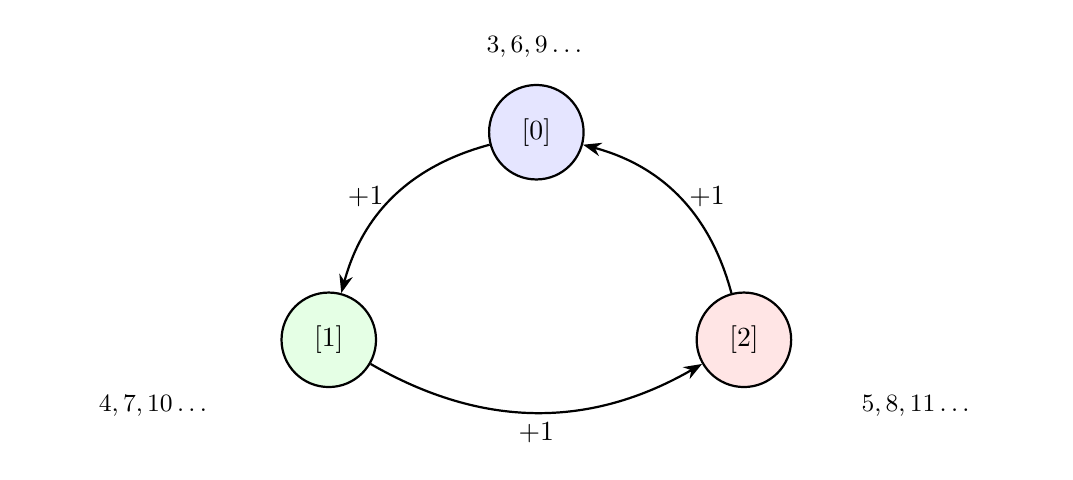
\begin{tikzpicture}[>=Stealth, node distance=2.5cm, auto, thick]
    % Nodes
    \node[circle, draw, minimum size=1.2cm, fill=blue!10] (0) { $[0]$ };
    \node[circle, draw, minimum size=1.2cm, fill=green!10] (1) [below left=of 0] { $[1]$ };
    \node[circle, draw, minimum size=1.2cm, fill=red!10] (2) [below right=of 0] { $[2]$ };
    
    % Edges for +1 operations
    \path[->] (0) edge [bend right=30] node [left] {$+1$} (1);
    \path[->] (1) edge [bend right=30] node [below] {$+1$} (2);
    \path[->] (2) edge [bend right=30] node [right] {$+1$} (0);
    
    % Labels
    \node[above=0.2cm of 0, text width=3cm, align=center] {\small $3, 6, 9 \dots$};
    \node[below left=0.2cm of 1, text width=3cm, align=center] {\small $4, 7, 10 \dots$};
    \node[below right=0.2cm of 2, text width=3cm, align=center] {\small $5, 8, 11 \dots$};
\end{tikzpicture}
\end{center}

\subsection{Heuristics \& ``Cheats''}
\begin{itemize}
    \item \textbf{The Exhaustion Heuristic:} If the modulus $n$ is small (e.g., $n \le 7$) and you are dealing with polynomials (like squares $x^2$ or cubes $x^3$), skip clever algebra and immediately map all $n$ cases. 
    \item \textbf{Negative Remainders Shortcut:} Note that $n - 1 \equiv -1 \pmod n$. For example, solving $6^{100} \pmod 7$ is trivial: $6 \equiv -1 \pmod 7 \implies (-1)^{100} = 1 \pmod 7$.
\end{itemize}

\subsection{Pitfalls \& Fallacies}
\begin{itemize}
    \item \textbf{The Division Trap:} You CANNOT arbitrarily divide in modular arithmetic! $ca \equiv cb \pmod n$ does NOT generally imply $a \equiv b \pmod n$ unless $\gcd(c, n) = 1$.
    \item \textbf{The Exponent Trap:} You CANNOT reduce exponents modulo $n$. That is, $a^{b} \pmod n \not\equiv a^{(b \bmod n)} \pmod n$. (Exponents are reduced using Euler's Totient function $\phi(n)$ via Fermat's/Euler's theorem).
\end{itemize}

% ==========================================
% PART 5: Conceptual Synthesis
% ==========================================
\newpage
\section{Part 5: Conceptual Synthesis and The ``Big Picture''}

\subsection{A) Thematic Connections}
The core theme of Section 4.2 is \textit{equivalence partitioning}. This creates an algebraic bridge between basic arithmetic and abstract set theory. By defining equivalence classes based on remainders, we take the infinite discrete sample space $\Omega = \mathbb{Z}$ and project it onto a compact, finite space $\Omega' = \mathbb{Z}_n$. This theme of "wrapping" a space back onto itself is conceptually identical to mapping random variables into bounded measurable spaces in measure theory.

\subsection{B) Forward and Backward Links}
\begin{itemize}
    \item \textbf{Backward Link:} This explicitly uses the well-ordering principle and the Division Algorithm from earlier introductory logic chapters.
    \item \textbf{Forward Link:} Congruence is the bedrock of Abstract Algebra. The sets $\mathbb{Z}_n$ form Cyclic Groups, Rings, and (when $n$ is prime) Fields. Furthermore, prime moduli behaviors are critical for Fermat's Little Theorem and the Euler Totient Theorem, which form the entire basis of modern Public-Key Cryptography (RSA).
\end{itemize}

% ==========================================
% PART 6: Abstract Real-World Modeling
% ==========================================
\newpage
\section{Part 6: Abstract Real-World Modeling (AI, ML, \& Quant Finance)}

\subsection{A) Concrete Scenarios}
\begin{enumerate}
    \item \textbf{Quantitative Finance - Monte Carlo Derivative Pricing:} To price exotic options without closed-form Black-Scholes solutions, analysts simulate millions of asset paths. Generating the massive arrays of random normal variables requires standard uniform distributions, which computationally rely on \textit{Linear Congruential Generators} (LCGs)—algorithms strictly governed by congruence relations.
    \item \textbf{Generative AI / Deep Learning - Locality-Sensitive Hashing (LSH):} AI models dealing with massive high-dimensional vector databases (like LLM embeddings) must perform fast nearest-neighbor searches. Hashing functions utilize large prime modulo arithmetic to deterministically bucket identical vectors without collisions.
\end{enumerate}

\subsection{B) Model Problem Setup: Stochastic Option Pricing via LCGs}

\textbf{Theoretical Framework:}
Consider an underlying asset in a risk-neutral measure space $(\Omega, \mathcal{F}, \mathbb{Q})$. The asset price $S_t$ follows Geometric Brownian Motion governed by the Stochastic Differential Equation (SDE):
\[ dS_t = r S_t dt + \sigma S_t dW_t \]
where $r$ is the risk-free rate, $\sigma$ is the volatility, and $W_t$ is a standard Wiener process. 

To simulate this via the Euler-Maruyama discretization scheme over intervals $\Delta t$, we must sample independent standard normal increments $Z \sim \mathcal{N}(0,1)$:
\[ S_{t+\Delta t} = S_t \exp\left( \left(r - \frac{1}{2}\sigma^2\right)\Delta t + \sigma \sqrt{\Delta t} Z \right) \]

\textbf{Generating $Z$ using Modular Arithmetic:}
True randomness is computationally impossible. We construct a pseudorandom state space using an LCG. Define a modulus $m$ (typically $2^{31}-1$, a Mersenne prime), a multiplier $a$, and an increment $c$. We generate a deterministic sequence of integers $X_k$ using the recurrence congruence:
\[ X_{k+1} \equiv (a X_k + c) \pmod m \]

For the sequence to achieve the maximum period $m$, it must satisfy the \textit{Hull-Dobell Theorem}, which states $c$ and $m$ are relatively prime, and $a - 1$ is divisible by all prime factors of $m$. 
We project these states into the continuous probability measure space $\mathcal{U}(0,1)$ via:
\[ U_{k+1} = \frac{X_{k+1}}{m} \]

Finally, we apply the Box-Muller transform to map our modulo-generated uniform space to the Gaussian domain required for the SDE:
\[ Z = \sqrt{-2 \ln(U_1)} \cos(2\pi U_2) \]

This model proves that without the rigorous algebraic structure of congruence over finite sets, computational stochastic calculus (and thus algorithmic trading simulations) would collapse.

% ==========================================
% PART 7: Common Variations and Untested Concepts
% ==========================================
\newpage
\section{Part 7: Common Variations and Untested Concepts}

The provided textbook section covers basic algebraic properties of congruence, but omits a critical proof archetype seen in advanced logic exams: \textbf{The Cancellation Law for Congruences}.

\textbf{Untested Concept:} Division in modular arithmetic. Students often erroneously assume that if $ca \equiv cb \pmod n$, they can divide by $c$ to get $a \equiv b \pmod n$. This is only true if $c$ and $n$ share no common factors (they are coprime).

\begin{theorem}[Cancellation Law]
Let $a, b, c, n \in \mathbb{Z}$ with $n \ge 2$. If $ca \equiv cb \pmod n$ and $\gcd(c, n) = 1$, then $a \equiv b \pmod n$.
\end{theorem}
\begin{proof}
\textbf{Proof Technique: Direct Proof using Bezout's Identity.} \\
Assume $ca \equiv cb \pmod n$. By definition, $n \mid (ca - cb)$, which means $n \mid c(a - b)$. 
Thus, there exists an integer $k$ such that:
\[ c(a - b) = nk \]
We are given that $\gcd(c, n) = 1$. By Bezout's Identity, there exist integers $x, y$ such that:
\[ cx + ny = 1 \]
Multiply both sides of Bezout's Identity by $(a - b)$:
\[ c(a - b)x + n(a - b)y = (a - b) \]
Substitute $c(a - b) = nk$ into the equation:
\[ (nk)x + n(a - b)y = a - b \]
Factor out the $n$ on the left side:
\[ n(kx + (a - b)y) = a - b \]
Since $k, x, a, b, y \in \mathbb{Z}$, the term $(kx + (a - b)y)$ is an integer. Thus, $n \mid (a - b)$, yielding:
\[ a \equiv b \pmod n \]
\end{proof}

% ==========================================
% PART 8: Advanced Diagnostic Testing
% ==========================================
\newpage
\section{Part 8: Advanced Diagnostic Testing: ``Find the Flaw''}

Below are five seemingly convincing mathematical proofs concerning congruence. Each contains a single, fatal logical flaw. Your task is to act as the grader: locate the flaw, explain the violation of the axioms, and reference the ``Solution Key'' to verify.

\begin{flawprob}
\textbf{Proposition:} If $6x \equiv 18 \pmod{12}$, then $x \equiv 3 \pmod{12}$. \\
\textit{Proof:} Assume $6x \equiv 18 \pmod{12}$. We recognize that both $6x$ and $18$ share a common factor of 6. Dividing both sides of the congruence by 6, we obtain $x \equiv 3 \pmod{12}$. $\blacksquare$
\end{flawprob}

\begin{flawprob}
\textbf{Proposition:} If $x \equiv 2 \pmod 4$ and $x \equiv 2 \pmod 6$, then $x \equiv 2 \pmod{24}$. \\
\textit{Proof:} Assume $x \equiv 2 \pmod 4$ and $x \equiv 2 \pmod 6$. By definition, $x = 4k + 2$ and $x = 6j + 2$. This implies that $x - 2 = 4k$ and $x - 2 = 6j$. Because $(x - 2)$ is a multiple of both 4 and 6, we multiply the moduli to find the combined state space, meaning $(x - 2)$ is a multiple of $4 \times 6 = 24$. Thus $x \equiv 2 \pmod{24}$. $\blacksquare$
\end{flawprob}

\begin{flawprob}
\textbf{Proposition:} $2^5 \equiv 2^2 \pmod 3$. \\
\textit{Proof:} We know that base congruence implies operational parity. Notice that for the exponents, $5 \equiv 2 \pmod 3$. Because the exponents belong to the same equivalence class modulo 3, we can substitute them in the base equation. Hence $2^5 \equiv 2^2 \pmod 3$. $\blacksquare$
\end{flawprob}

\begin{flawprob}
\textbf{Proposition:} If $x^2 \equiv 1 \pmod 8$, then $x \equiv 1 \pmod 8$ or $x \equiv -1 \pmod 8$. \\
\textit{Proof:} Assume $x^2 \equiv 1 \pmod 8$. Subtracting 1 from both sides yields $x^2 - 1 \equiv 0 \pmod 8$. Factoring the difference of squares gives $(x - 1)(x + 1) \equiv 0 \pmod 8$. By the zero-product property of algebra, if the product of two factors is zero, at least one factor must be zero. Therefore, $x - 1 \equiv 0 \pmod 8 \implies x \equiv 1 \pmod 8$, or $x + 1 \equiv 0 \pmod 8 \implies x \equiv -1 \pmod 8$. $\blacksquare$
\end{flawprob}

\begin{flawprob}
\textbf{Proposition:} For any positive integer $n \ge 2$, if $ab \equiv 0 \pmod n$, then $a \equiv 0 \pmod n$ or $b \equiv 0 \pmod n$. \\
\textit{Proof:} Assume $ab \equiv 0 \pmod n$. By definition, $n \mid (ab)$. Since divisibility distributes across multiplication, the divisor $n$ must divide the first term $a$, or it must divide the second term $b$. Therefore, $n \mid a \implies a \equiv 0 \pmod n$, or $n \mid b \implies b \equiv 0 \pmod n$. $\blacksquare$
\end{flawprob}

\vspace{2cm}

\subsection*{Solution Key to Diagnostic Problems}
\begin{itemize}
    \item \textbf{Problem 1 Flaw:} \textit{Illegal Division.} You cannot divide a congruence relation by a constant unless that constant is coprime to the modulus ($\gcd(6, 12) \neq 1$). The true relation would divide the modulus as well: $x \equiv 3 \pmod{2}$.
    \item \textbf{Problem 2 Flaw:} \textit{False Modulus Multiplication.} If a number is a multiple of $a$ and $b$, it is a multiple of their \textit{least common multiple} (LCM), not necessarily their product. $\operatorname{lcm}(4, 6) = 12$. The correct conclusion is $x \equiv 2 \pmod{12}$. (Counterexample for 24: $x=14$).
    \item \textbf{Problem 3 Flaw:} \textit{Exponent Fallacy.} Congruences DO NOT apply to exponents. The proof attempts to substitute exponents, which is invalid. To see why, mathematically $2^5 = 32 \equiv 2 \pmod 3$, while $2^2 = 4 \equiv 1 \pmod 3$. $2 \not\equiv 1 \pmod 3$. 
    \item \textbf{Problem 4 Flaw:} \textit{Applying Real-Number Properties to Non-Prime Rings.} The ``Zero-Product Property'' strictly requires an integral domain (which $\mathbb{Z}_8$ is not, because 8 is not prime). In $\mathbb{Z}_8$, factors can multiply to zero without either being zero (e.g., $2 \times 4 \equiv 0 \pmod 8$). (Counterexample: $x=3 \implies 3^2 = 9 \equiv 1 \pmod 8$).
    \item \textbf{Problem 5 Flaw:} \textit{Prime Divisibility Axiom Misapplication.} The claim ``if $n \mid ab$ then $n \mid a$ or $n \mid b$'' is Euclid's Lemma, which is STRICTLY true only if $n$ is a prime number. If $n$ is composite, it can be constructed by parts of $a$ and $b$. (Counterexample: $n=6, a=2, b=3 \implies 6 \mid (2 \times 3)$, but $6 \nmid 2$ and $6 \nmid 3$).
\end{itemize}

\end{document}